\documentclass[9pt,twocolumn,twoside]{gsajnl}

\include{hyperref}

\articletype{inv} % article type
% {inv} Investigation 
% {gs} Genomic Selection
% {goi} Genetics of Immunity 
% {gos} Genetics of Sex 
% {mp} Multiparental Populations

\title{Microarray-based detection of genomic signatures related with the tumor recurrence in Glioblastoma patients}

\author[$\ast$,1]{Álvaro Abella-Bascarán}
\author[$\ast$]{Eloi Casals-Puig}
\author[$\ast$]{Samuel Miravet-Verde}

\affil[$\ast$]{Pompeu Fabra University, Barcelona (Spain)}

\keywords{Microarray; tumour recurrence; glioblastoma.}

\runningtitle{GENETICS | INVESTIGATION}

\correspondingauthor{Corresponding Author}

\begin{abstract}

Regretfully glioblastomas are notorious for resistance to therapy (and consequently for their recurrence), which has been attributed to DNA-repair proficiency, a multitude of dysregulated molecular pathways, and, more recently, to the particular...

With the different approach for the analysis of the reference data, we see that recurrence is far from being attributed to few pathways, and it must be seen as the consequence of a combination of multiple over and underexpressed molecular routes. Between all of them, we can highlight, for the recurrent patients, an expression profile characterized by differentially expressed genes to give the ability to escape immune response and apoptosis, along with an upregulation of cycle and division processes, favored with a higher metabolic demand. 

All the features exposed in this article, in addition to those presented by the original work of Anastasia Murat \citep{Murat2008}, represent specific genetic features of recurrent tumors. This profile can have a important clinical interest as it suppose a simple method to detect those potential recurrent tumors and adjust the treatments to avoid a possible relapse.


\end{abstract}

\setboolean{displaycopyright}{true}

\begin{document}

\maketitle
\thispagestyle{firststyle}
\marginmark
\firstpagefootnote
\correspondingauthoraffiliation{Affiliation correspondence email:  alvaro.abella01@estudiant.upf.edu}

\vspace{-1cm}
\section*{\underline{Introduction}}


%Linkear HTML del supplementary matherial en todo lo que lo diga

Glioblastoma multiforme, involving glial cells, is the most frequent and aggressive brain tumor in humans, with an incidence of 2–3 cases per 100,000 person life-years in Europe and North America \citep{Bleeker2012}. Its treatment can involve chemotherapy, radiation and surgery. Median survival with standard-of-care radiation and chemotherapy with the alkylating agent temozolomide is only 15 months  \citep{Johnson2012} while the median survival without treatment is 4 and a half months. 

Regretfully glioblastomas are notorious for resistance to therapy (and consequently for their recurrence). The treatment for this cases requires a more aggressive combination of drugs, including nitrosoureas, temozolomide, bevacizumab, in addition to radiotherapy \citep{Weller2013}. This approach implies several risks for the patient and, therefore, it is only applied after the relapse of the patient.

Biologically, the recurrence has been initially attributed to DNA-repair proficiency, cell proliferation and, more recently, to the particular biologic behavior of tumor stem-like cells, as it is exposed in the work of Anastasia Murat \citep{Murat2008}. In that case the HOX and EGFR related pathways were identified as the most differentially expressed using clustering techniques and rigid statistical methods. We propose here a deeper analysis, based on more general techniques, to determine the molecular profiles specific for recurrent tumours.

\section*{\underline{Materials and Methods}}

\subsection*{Tumor Samples and Patient Characteristics}

We analyzed data from 80 frozen glioblastoma samples. The data comprised 70 tumors from initial surgery and 10 samples resected at recurrence. All patients were treated within a phase II or a randomized phase III trial \citep{Stupp2002,Stupp2005}
The study includes 21 females and 55 males, with a a median age of 52 (range, 26 to 70 years). Out of the 76 patients, 28 received radiotherapy treatment only, and 48 received TMZ/radiotherapy treatment.

\subsection*{Gene Expression Profiling}

The microarray data with gene expression profiling was obtained from the Gene Expression Omnibus (GEO) database at \url{http://www.ncbi.nlm.nih.gov/geo/} (accession-number GSE7696). The data had been created from probes prepared with the Enzo BioArray-High Yield Kit (Enzo Life Sciences, Farmingdale, NY) for double amplification and were hybridized to Affymetrix HG-133Plus2.0 GeneChips (Affymetrix, Santa Clara, CA). The data used had been normalized to the expression of the EIF2C3, DNAJA4, and B2M genes that exhibited little variation in the data set \citep{Murat2008}.

\subsection*{Data Analysis and Statistical Methods}
Analyses were carried out in R, a free software environment available at \url{http://www.r-project.org/}. The full list of packages and modules used can be found in te session information part at the end of the supplementary document. 

\subsubsection*{Quality assessment:}
the quality of the microarray data was assessed by a variety of quality checks. Raw chip images were visually inspected to ensure the absence of  artifacts. The intensity distributions of the samples showed a similar poisson distribution, without any artifactual distribution. We used the linear probe level model (PLM) \citep{Bolstad2004, Brettschneider2007} to verify the absence of artifacts in the chip pseudoimages created from the weights and residuals of the sample PLM's. We used Normalized Unscaled Standard Errors (NUSE) \citep{Bolstad2004} to evalute the deviation of the chip probsets. Samples with NUSE median value higher than 1.05 were removed. Using the same models, we also evaluated the Relative Log Expression (RLE) values \citep{Bolstad2004, Brettschneider2007} to determine technical biases on particular chips. No particular deviation of the median or the interquartile range was found on any sample. The expression intensities for all probe sets from Affymetrix CEL-files were estimated using robust multiarray average  with probe-level quantile normalization followed by median polish summarization \citep{Irizarry2003} as implemented in the BioConductor software (\url{http://www.bioconductor.org/}). The inspection of MA plots ensured the absence of fluorescent intensity dependent biases \citep{Bolstad2004}. After the quality assurance process, no samples were discarded from the analysis.

\subsubsection*{Analysis of batch effect and confounding variables:}
the samples were checked for batch effect, first using hierarchical clustering after measuring the Spearman correlation among samples, and then verifying the absence of batch effects by multidimensional scaling. The presence of confounding variables was assessed by means of principal component analysis, and different sources of heterogeneity were analyzed by surrogate variable analysis \citep{Leek2007}.

\subsubsection*{Differential Expression}: the list of analyzed probes was reduced using a non-specific filtering \citep{Bourgon2010}, eliminating features with little variation (IQR cutoff = 0.5), consistently low signal across samples, or insufficient annotation. The differential expression analysis of microarray data was done with an empirical Bayes method \citep{Smyth2004} implemented in the Bioconductor package limma. The Benjamini-Hochberg procedure was applied for multiple testing correction (false-discovery rates) \citep{Benjamini1995}. We called Differentially Expressed (DE) genes at 10\% FDR.

\subsubsection*{Functional Enrichment}: we analysed the enrichment of gene ontology terms (\url{http://www.geneontology.org}) for biological processes (GO BP) using a one-tailed Fisher's exact test \citep{Fisher1922}. The significance of the GO terms is computed conditionally to the significance of its child terms \citep{Alexa2006}. GO terms formed by less than five genes or with less than five DE genes were removed to improve the reliability of the results. This concrete analysis was repeated three times, one considering DE genes in general and two more with only overexpressed and underexpressed genes in the recurrent patients. 

\subsubsection*{Simple GSEA}: Gene Set Enrichment Analysis \citep{Subramanian2005} was carried out using the simple GSEA algorithm \citep{Irizarry2009}, as provided in the \href{http://www.bioconductor.org/packages/release/bioc/html/GSEABase.html}{GSEABase} package from the Bioconductor project. The gene sets used during the analysis are the ones available in the package \href{http://www.bioconductor.org/packages/release/data/experiment/html/GSVAdata.html}{GSVAdata}, with the name `c2BroadSets', once restricted to those which belong to pathways from \href{http://www.genome.jp/kegg/pathway.html}{KEGG}, \href{http://www.reactome.org/}{REACTOME} and \href{http://www.biocarta.com/}{BIOCARTA}. In order to add some robustness to the calculation of the Z-scores, the evaluation was limited to gene sets having 5 or more genes. Finally, only gene sets with an FDR of less than 10 \% were called differentially expressed.

\subsubsection*{Work flow and scripts}: in order to ensure the reproducibility of results, all the analysis steps performed can be found in the supplementary material in \textit{HTML} format. This file was processed directly from R using 
\href{http://cran.r-project.org/web/packages/knitr/index.html}{knitr} and \href{http://cran.r-project.org/web/packages/markdown/index.html}{markdown}. The file contains detailed explanations about the methodology, statistical interpretation and graphics generated during the process. 


\section*{\underline{Results and Discussion}}

The analysis of differential expression show 255 genes differentially expressed (ref. a volcano plot) (corrected p-value < 0.1) across the two conditions (recurrent and non-recurrent GBM). From this set of genes we performed the Gene Ontology (GO) enrichment analysis in general and dividing by under and overexpressed genes in recurrent data. Additionally, a simple GSEA was carried out to check similarities and possible new pathways DE. The results of the analysis developed are presented below including some biological inferences. The GO enrichment analysis are exposed in three different subsection and at the end the results of the GSEA can be found.\\
A general overview of the results obtained can be found in the table \ref{tab:resume}.

\begin{figure}[!h]
	\centering
	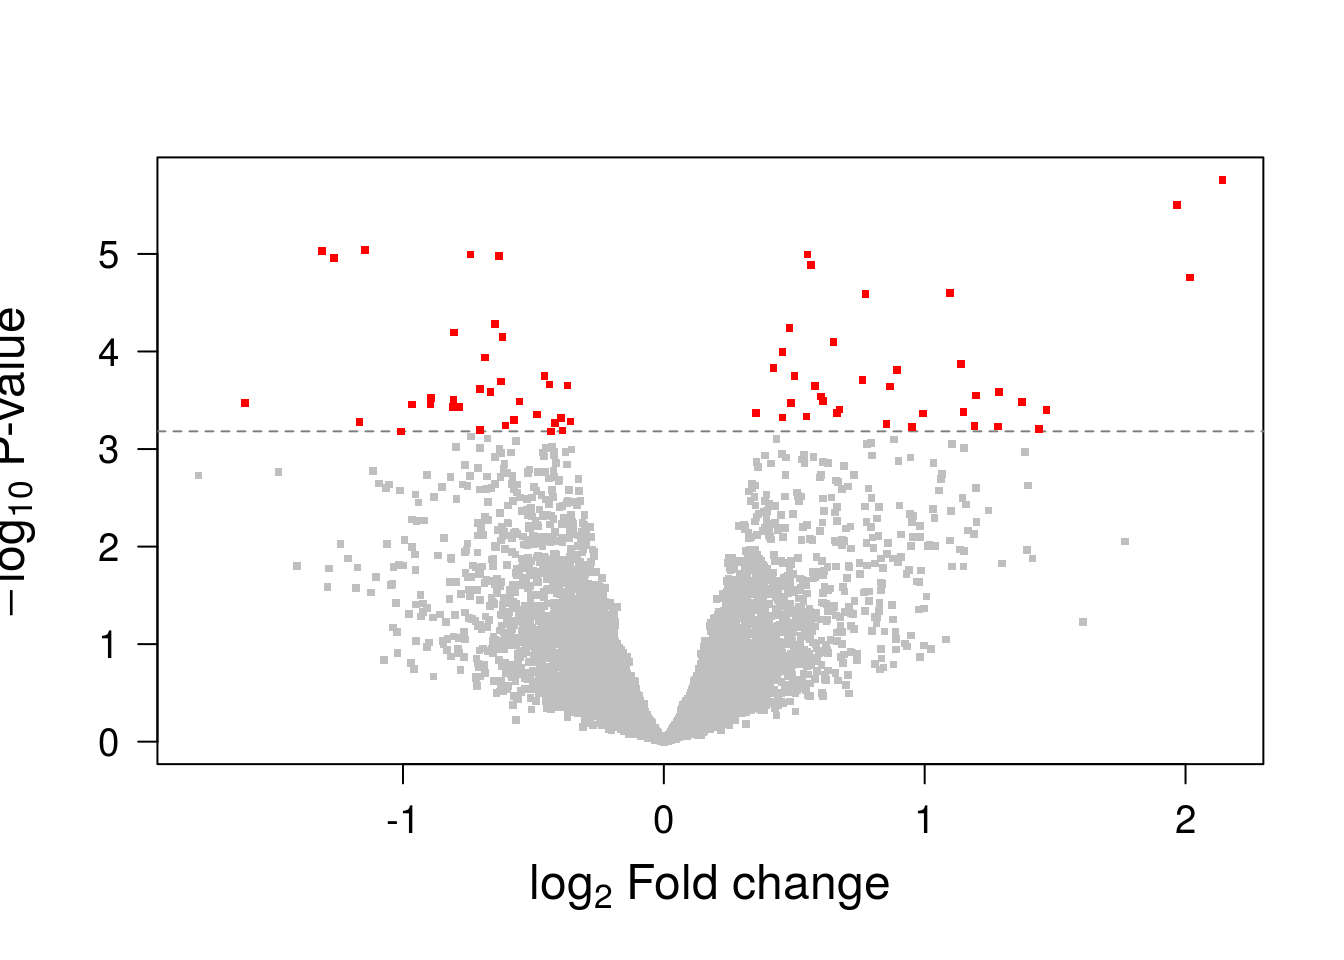
\includegraphics[scale=0.4]{volcano.png}
	\caption{Volcano plot showing DE genes (red), with negative and positive fold changes indicating underexpressed and overexpressed genes, respectively, in recurrent tumours.}
	\label{fig:volcano}
\end{figure}


\begin{table*}[!htbp]
\centering
\caption{\bf Resume of results}
\begin{tableminipage}{\textwidth}
\begin{tabularx}{\textwidth}{m{3.4cm}m{2.6cm}m{1.5cm}m{9.2cm}}
\hline
Condition & Number of terms\footnote{Gene Ontology terms or Pathway terms} & nº genes & Important functions included\\
\hline

General GO Enrichment & 43 & 161 & Metabolic processes, Regulation of differentiation, Immune response, Intracellular transport, Extracellular transport \& Homeostasis, negative regulation of cell cycle G1/S phase transition, Cell adhesion, Anatomical cell structure, Protein modification. \\

Underexpression GO Enrichment & 15 & 66 & Cell surface, Negative regulation of cell cycle, proliferation \& apoptisis, Immune response, Cell adhesion, RNA processing, Negative regulation of protein transport.\\

Overexpression GO Enrichment & 34 & 116 & Negative regulation of cell death \& apoptosis, Metabolic processes, Cell structure organization, Transport and Homeostasis, DNA \& Protein modification, Immune response \& Inflammation.\\

Gene Set Enrichment Analysis & 32 & 45 & ATG10, SNF8, RPS9, BAX, TIMM17A, PRMT1, PIN1, OGT, PSMD4, OGT , FBXW7, PSMC1, HNMT, RPL27A, DPH5, CYR61, GSTP1,  PCMTD1, PSMD3,  CTNNB1, ASB1, PEX16,  SEC31A,PIN1, RGS4, MYDGF, TRIP6, CTNNB1, HOMER3, CCL5 , WDR46, CCNB1IP1\\

\hline
\end{tabularx}
  \label{tab:resume}
\end{tableminipage}
\end{table*}

\subsubsection*{General Enrichment}:The GO enrichment revealed 43 enriched terms (table can found in the supplementary matherial) when considering together under and overexpressed genes. In total, 161 genes significantly differentially expressed were included in this group.\\
The enrichment include terms related to metabolic processes (eg. glucose metabolic process and hexose biosynthetic process), immune response (eg. regulation of T-cell activation and regulation of lymphocyte proliferation), and cell proliferation (regulation of cell cycle G1/S phase transition and regulation of cell proliferation).\\
This profile suggests that glioblastoma recurrence is due to heterogeneous causes, possibly combining a higher ability to escape immune response with an even more dysregulated cell cycle, supported by a higher glucose metabolism.

\subsubsection*{Underexpression Enrichment}: the enrichment with underexpressed DE genes revealed 66 different grouped in 15 GO terms (table \ref{tab:under}), among which we can highlight the `apoptotic signaling pathway'. It is known that defects in apoptosis signalling contribute to tumor resistance \citep{Debatin2004}, and we can therefore include it as a feature contributing to recurrence in glioblastoma. This situation of resistance and growth uncontrolled is also favored by the downregulation of pathways related negatively with the proliferation and cell cycle control.\\
In addition, it is interesting to remark the bigger set of genes, 29, presented by the `Cell surface receptors pathways'. This could be related with fact that cancerous cells inhibit the exposure of death receptor to their surface in addition to other possible antigen that could be detected by the immune system \citep{Ozoren2003}.

\subsubsection*{Overexpression Enrichment}: the enrichment done with overexpressed DE genes in recurrent patients revealed 34 different GO terms (table \ref{tab:over}) including in total 116 different genes. An interesting result are the enriched terms of `exocytosis' and `transport proteins' (both included in the class `Transport and Homeostasis').\\
Respect the exocitosis, as it is known that invasion by cancer cells is facilitated by the secretion of enzymes that degrade the extracelular matrix, and that glioma invasion can be inhibited through inhibition of exocytosis \citep{Liu2012}. Recurrence of the tumor could thus be related with a higher capacity to invade new areas.\\
On the other hand, about the `Transport proteins', one of the most common types of cancer resistance consists in the overexpression of drug pumps able to expel the chemotherapeutical drugs from the cell \citep{Borst2012}. The overexpression of proteins with transmembrane transport function could be related with the recurrence as the tumor cells were throwing out the temozolomide drug.
% TODO mirar si alguna de esas proteines se encuentra en nuestra lista.

\subsubsection*{Gene Set Enrichment Analysis}:

\section*{\underline{Conclusion}}
In the paper where the data was extracted \citep{Murat2008} the differentially expressed genes related with the survival of the patients were those participating in DNA-repair proficiency and stem-like behaviour (HOX and EGFR). Here, we have extended their results studying the genetic profile of recurrent patients of glioblastoma. The general overview of results shows clearly the recurrence cannot be attributed to a single pathway and it must be seen as the consequence of a multiple set of features, among which we can highlight a higher ability to escape immune response and apoptosis, and a more dysregulated cell cycle and monosacharyde metabolism, all of the overexpressed respect the non-recurrent profile.

As this study is a comparison of recurrent and non-recurrent glioblastoma, we do not dispose of information to know whether this pathways are also enriched in the case of glioblastoma with respect to controls. This information would be useful to draw conclusions about whether recurrence is a consequence of a qualitatively different expression profile, or a quantitative matter (simply a consequence of higher expression of cancer-related pathways).

In conclusion, this article exposes a statistically significant genetic profile related with the relapse of glioblastoma patients due to the recurrence of the tumor. As the glioblastoma is one of the most recurrent types of cancer \citep{Bleeker2012}, the definition of a concrete expression profile opens the possibility of having a way to prevent and detect the potential recurrent patients in order to personalize the treatment with the current approaches to recurrent tumors \citep{Weller2013}. 

\section*{Figures and Tables}

Figures and Tables should be labelled and referenced in the standard way using the \verb|\label{}| and \verb|\ref{}| commands.

\subsection*{Sample Figure}

Figure \ref{fig:spectrum} shows an example figure.

\begin{figure}[htbp]
\centering
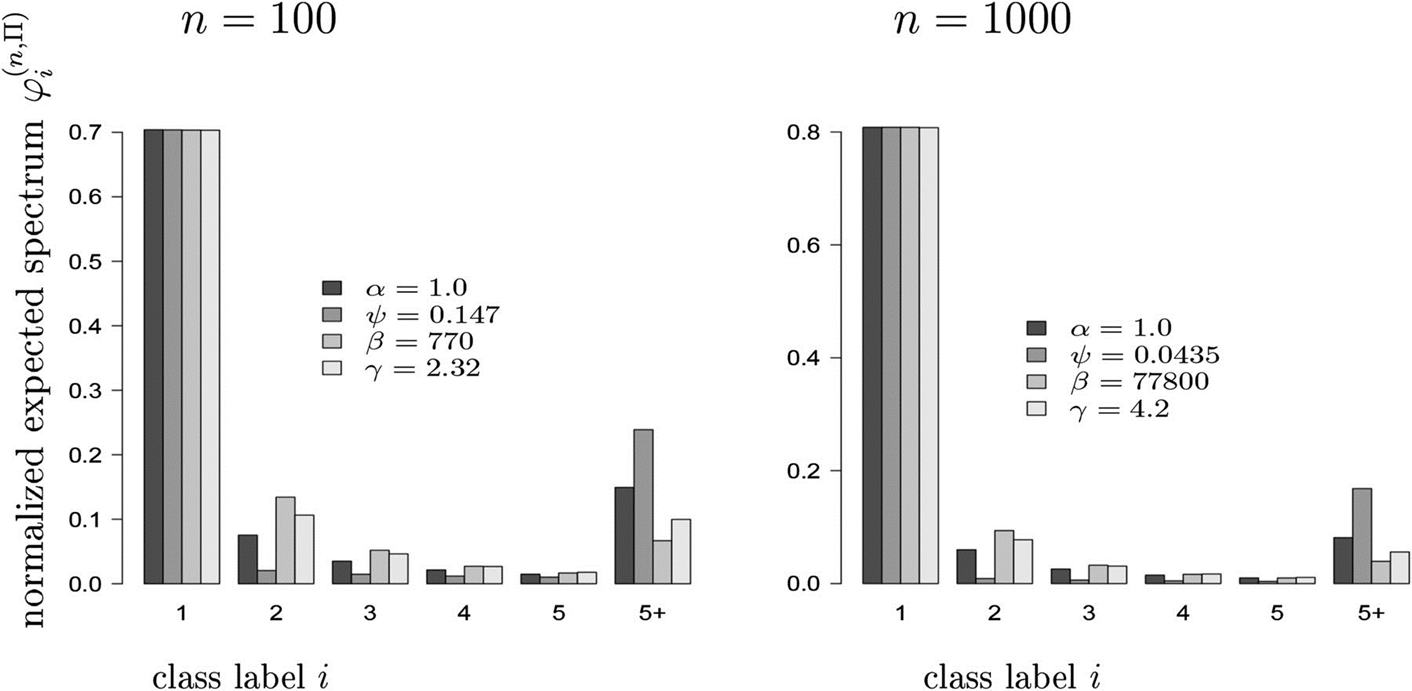
\includegraphics[width=\linewidth]{example-figure}
\caption{Example figure from \url{10.1534/genetics.114.173807}. Please include your figures in the manuscript for the review process. You can upload figures to Overleaf via the Project menu. Upon acceptance, we'll ask for your figure files to be uploaded in any of the following formats: TIFF (.tiff), JPEG (.jpg), Microsoft PowerPoint (.ppt), EPS (.eps), or Adobe Illustrator (.ai).  Images should be a minimum of 300 dpi in resolution and 500 dpi minimum if line art images.  RGB, CMYK, and Grayscale are all acceptable. Halftones should be high contrast with sharp detail, because some loss of detail and contrast is inevitable in the production process. Figures should be 10-20 cm in width and 1-25 cm in height. Graph axes must be exactly perpendicular and all lines of equal density.
Label multiple figure parts with A, B, etc. in bolded type, and use Arrows and numbers to draw attention to areas you want to highlight. Legends should start with a brief title and should be a self-contained description of the content of the figure that provides enough detail to fully understand the data presented. All conventional symbols used to indicate figure data points are available for typesetting; unconventional symbols should not be used. Italicize all mathematical variables (both in the figure legend and figure) , genotypes, and additional symbols that are normally italicized.  
}%
\label{fig:spectrum}
\end{figure}



\begin{figure}[htbp]
\centering
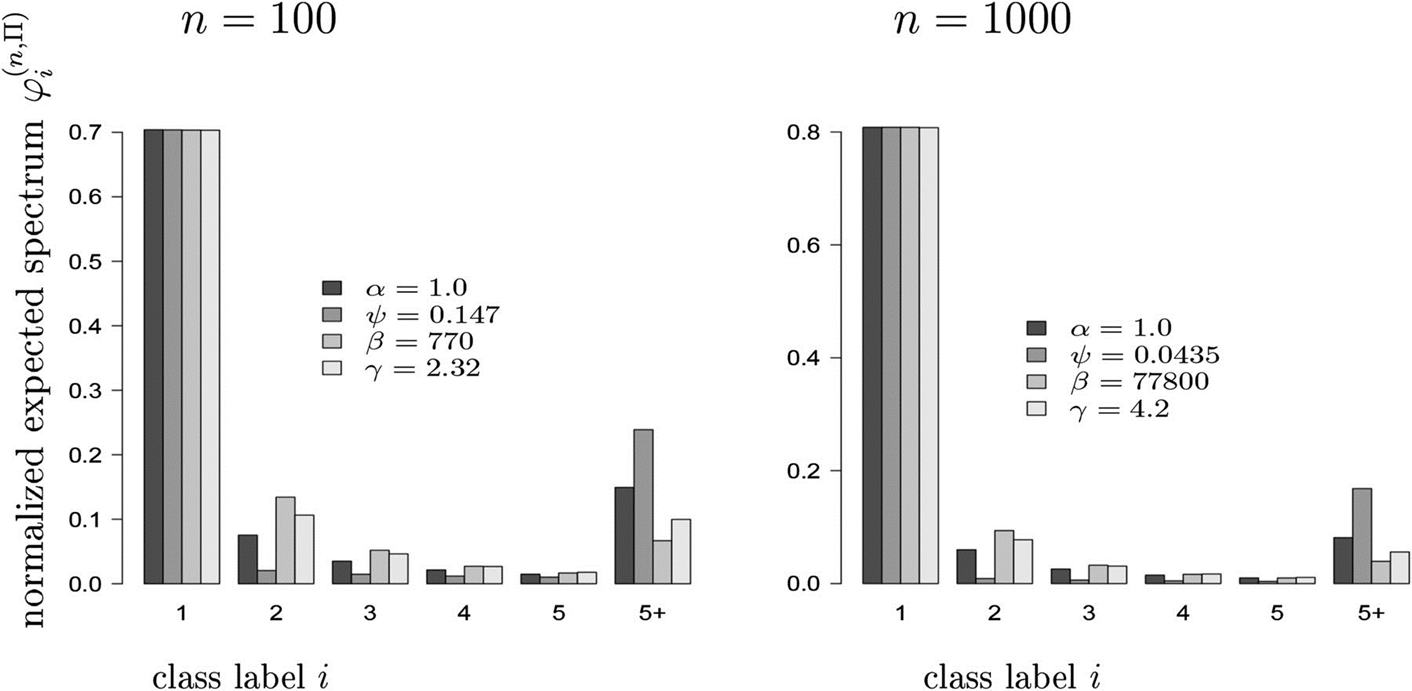
\includegraphics[width=\linewidth]{example-figure}
\caption{Example movie (the figure file above is used as a placeholder for this example). \textit{GENETICS} supports video and movie files that can be linked from any portion of the article - including the abstract. Acceptable formats include .asf, avi, .wav, and all types of Windows Media files.   
}%
\label{video:spectrum}
\end{figure}

\bibliography{example-bibliography}


\begin{table*}[htbp]
\centering
\caption{\bf Underexpressed Genes}
\begin{tableminipage}{\textwidth}
\begin{tabularx}{\textwidth}{m{3cm}m{3.5cm}m{1.2cm}m{9.2cm}}
\hline
Biological Processes & GOBPID terms & nº genes & Genes included\footnote{Genes can overlap between GO terms.} \\
\hline

Cell surface receptors pathways & GO:0007166 & 29 & ACTR2, LILRB1, CYLD, ATP6V0E2, EFNB2, CCNY, PEG10, NPB, ADGRD1, TMEM145, IFNGR1, ITGB8, KRAS, NCK1, PDPK1, PRKACB, BIRC6, CEACAM1, RGS18, BMP2, TIAM1, CA2, CPEB4, DYRK2, CBL, KAT2B, ACVR1B, USP34, P2RY14\\

Negative regulation of cell cycle, proliferation \& apoptosis& GO:0051726, GO:0008285, GO:0097190 & 23 & TMOD3, FABP7, LILRB1,TOM1L1, CD33, PRPF40A, DYRK2, NCK1, PRKACB, CYLD, EFNB2, PDPK1, NACC2, ARL6IP5, BIRC6, RBL2, CCNY, TIAM1, SF1, KAT2B, CTBP1, ACVR1B , BMP2\\

Immune response \& Cell Adhesion & GO:0045088, GO:0051249, GO:0002684, GO:0006955, GO:1903037, GO:0034110  & 16 & PDPK1, CYLD, SUSD4, TLR5, CA2, ACTR2, SPPL2A, LST1, HAMP, LILRB1, PRKACB, IFNGR1,LILRB1, ACVR1B, SASH3, NCK\\

Regulation of hydrolase activity & GO:0051336 & 14 & ARL6IP5, CST3, ITSN2, ASAP1, PDPK1, SERPINB6, PRKACB, BIRC6, ARHGAP9, RGS18, BMP2, WNK1, TIAM1, DENND1C\\ 

RNA processing & GO:0006396 & 9 & SRRM1, PAPD4, DHX36, HNRNPA2B1, PRPF40A, RP9, SF1, SLBP, SCAF11\\

Axon Guidance & GO:0007411 & 7 & ACTR2, EFNB2, KIF5C, KRAS, NCK1, TIAM1, ZIC2\\

Negative regulation of protein transport & GO:0051224 & 5 & LYPLA1, LILRB1, CYLD, RHBDF2, DYRK2\\

Activation of protein kinase activity & GO:0032147 & 5 & TOM1L1, KRAS, PDPK1, PRKACB, BMP2\\
\hline
\end{tabularx}
  \label{tab:under}
\end{tableminipage}
\end{table*}

\pagebreak
 

\begin{table*}[htbp]
\centering
\caption{\bf Overexpressed Genes}
\begin{tableminipage}{\textwidth}
\begin{tabularx}{\textwidth}{m{3cm}m{3.5cm}m{1.2cm}m{9.2cm}}
\hline
Biological Processes & GOBPID terms & nº genes & Genes included\footnote{Genes can overlap between GO terms.} \\
\hline

Metabolic Processes & GO:1903050  GO:0042180  GO:0045862  GO:0034655  GO:0005996  GO:0006066  GO:0044265  GO:0043085, GO:0043170 & 82 &  RPP30, ASB1, RTCB, ZNF397, NRBP1, U2AF1, PIGC,  CYR61,  FUCA1, CFH, FBXW7, PCMTD1, PSMD4, CCL5, MAN1B1, PRMT1, MYDGF, COL12A1, SEC31A, PSMC1, DRG1, RPL27A, ATG10, ZNF554, PSMD3, APOL2, TRAPPC2, GSTP1, CYR61,  PMVK, WDR46, FUCA1, CCNB1IP1, BAX, DIS3, STX12, ZNF426, APOL3, SLC35D2, PTGER3, SLC35B4, CTNNB1, RETSAT, RPS9, POLR3GL, RGS4,  FBXW7, SAMD4B, NPY1R, EIF6, USP7, USP7 , INPPL1, TRIP6, PPAP2A,  SEC31A, LIG4, POLR3C, ZCCHC11, ATF5, MFAP4, TOB2, OGT,  PDE10A,TIMM17A, OSR2, ZBTB26, CCS, ZNF791, PIN1, NUDT4, CTSD, DPH5, COPS6, CCL8, RPE65, SNF8, ZNF496,  MAN1B1, OBFC1, APOBEC3F, RPA2\\

Cell structure organization & GO:0043062, GO:0044419, GO:0051234, GO:0051640 & 54 & APOL2, NUDT4, CALU, SLC39A7, CCL8,COL12A1, USP7, EIF6, TMED9, ECM2, BAX, CYR61, ABI3BP, ATG10, CCS, APOL3, SEC31A, ANTXR2, TRAPPC2, CCL5, TRIP6, HNMT, SLC35B4, INPPL1, TIMM17A, TMEM63A, NRBP1, COPS6, PSMC1, SNF8, FBXW7, HOMER3, MCOLN2, STX12, PTGER3, SYTL5, PSMD3, SNCAIP, PSMD4, RPL27A, CTNNB1, CTSD, RPS9, PEX16, RIMS4, WDR46, U2AF1, SLC26A7, ARF5, LIG4, SLC35D2, MFAP4, APOBEC3F\\

Transport and Homeostasis & GO:0006887, GO:0016482, GO:0006816, GO:0072511, GO:0060249,  GO:0051650, GO:0044765 & 43 & SLC35B4, TMEM63A, U2AF1, HOMER3, SLC39A7, MCOLN2, WDR46, OBFC1,  COPA, SLC26A7, CCS  , TMED9, EIF6, COPA, NRBP1, TIMM17A, APOL2, CALU, SYTL5, NUDT4, SLC35D2, SNCAIP, SNF8,SNF8, SEC31A, RPL27A, BAX, SYTL5  TIMM17A, STX12, RPS9, CTNNB1, CCL5, APOL3, HNMT,  CTNNB1, CCL8, TRAPPC2, TRIP6, RPA2, RPE65, RIMS4, PEX16, PTGER3\\

DNA \& Protein Modification & GO:1903322, GO:0032259, GO:0031400, GO:0006605, GO:0032446, GO:0051338 & 32 & ATG10, SNF8, RPS9, BAX, TIMM17A, PRMT1, PIN1, OGT, PSMD4, OGT , FBXW7, PSMC1, HNMT, RPL27A, DPH5, CYR61, GSTP1,  PCMTD1, PSMD3,  CTNNB1, ASB1, PEX16,  SEC31A,PIN1, RGS4, MYDGF, TRIP6, CTNNB1, HOMER3, CCL5 , WDR46, CCNB1IP1\\

Immune Response \& Inflamation & GO:0002478, GO:0019882, GO:0016032, GO:0001817, GO:0006954  & 28 & CFH, PSMD3, GSTP1, FBXW7, RPS9,  COPS6, PSMC1, POLR3GL,  APOL2, ASB1, SNF8, APOBEC3F, PSMD4,CTSD, BAX, ZCCHC11, RPL27A,  POLR3C, LIG4,  CTSD, PTGER3, APOL3  , USP7, PIN1, SEC31A, CTNNB1, CCL8, CCL5\\

Negative regulation of apoptosis \& cell death & GO:0030111, GO:0060548, GO:0043066  & 15 & MYDGF, CYR61,  CTNNB1,WIF1, CCL5, PSMC1,  ATF5, BAX, PSMD3, CTNNB1, GSTP1, PSMD4, LIG4, ATF5, CCL5\\

\hline
\end{tabularx}
  \label{tab:over}
\end{tableminipage}
\end{table*}





\end{document}
